%!TEX root = main.tex

\newpage
\appendix


\vspace*{\fill}
\begin{center}
	\section{Appendix}
\end{center}
\vspace*{\fill}

\newpage
\begin{landscape}
\global\pdfpageattr\expandafter{\the\pdfpageattr/Rotate 90}

\subsection{Appendix A - Gantt diagrams} \label{App:A}

% \begin{figure}[!ht]
% \begin{center}
% \caption{\small \sl First semester gantt.\label{fig:gantt1}}
% \end{center}
% \end{figure}

\begin{figure}[!ht]
\begin{center}
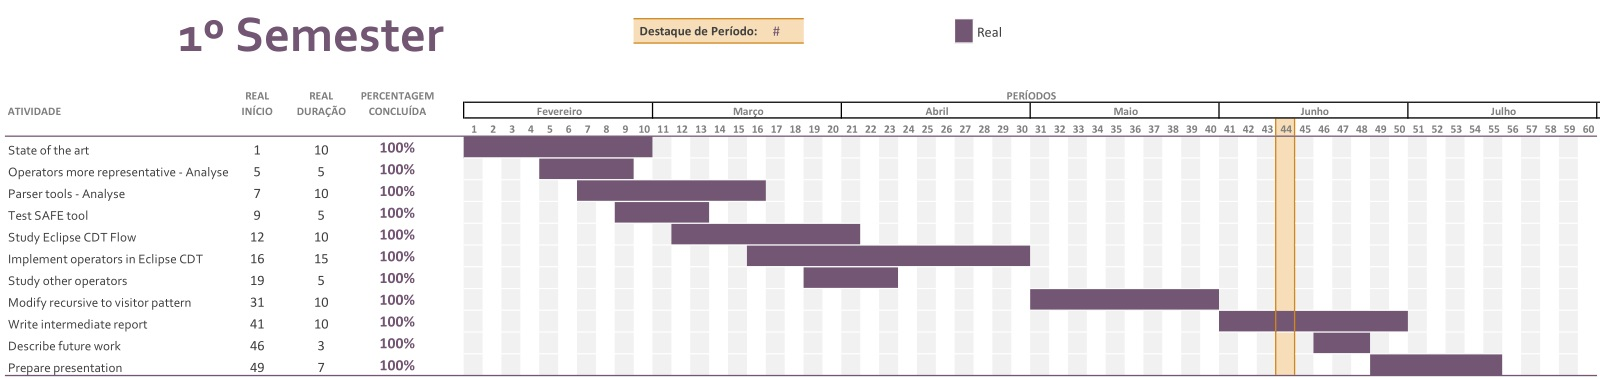
\includegraphics[width=1.6\textwidth]{gantt1.jpg}
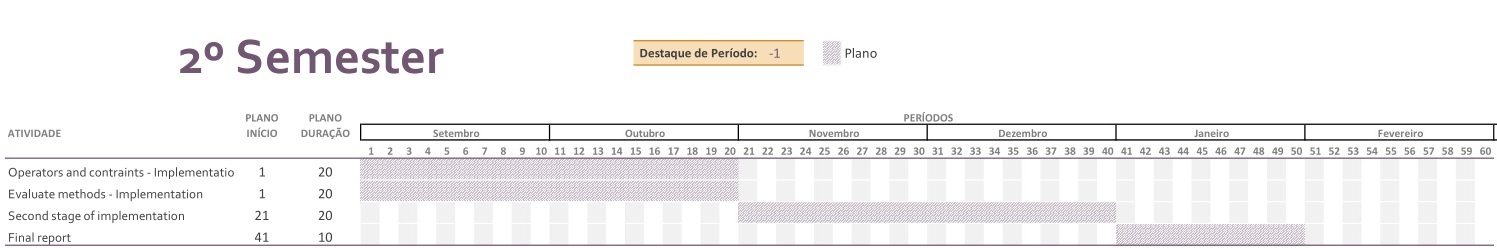
\includegraphics[width=1.6\textwidth]{gantt2.jpg}
\caption{\small \sl First and second semester gantt.\label{fig:gantt}}
\end{center}
\end{figure}

\clearpage

\subsection{Appendix B - Risks table} \label{App:B}
\begin{figure}[!ht]
\begin{center}
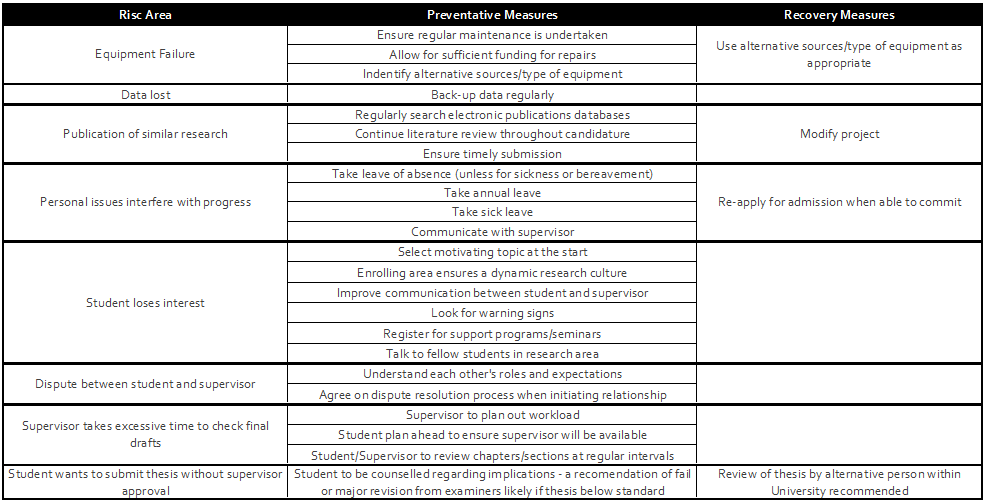
\includegraphics[width=1.5\textwidth]{risks.png}
\caption{\small \sl Risks.\label{fig:risks}}
\end{center}
\end{figure}

\end{landscape}
\global\pdfpageattr\expandafter{\the\pdfpageattr/Rotate 0}

\clearpage

\newpage
\subsection{Appendix C - Decision Tree} \label{App:C}
\begin{figure}[!ht]
\begin{center}
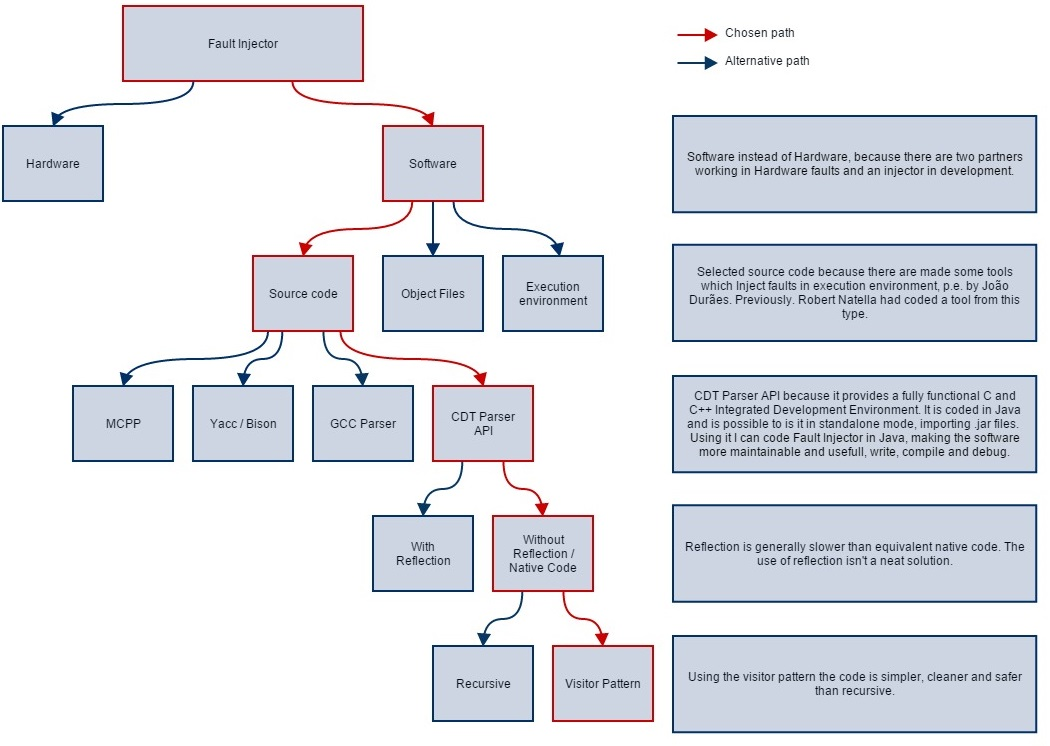
\includegraphics[width=1.1\textwidth]{decisions.jpg}
\caption{\small \sl Decision Tree.\label{fig:decisions}}
\end{center}
\end{figure}



\newpage
\subsection{Appendix D - Abbreviations} \label{App:D}
% \addcontentsline{toc}{section}{Abbreviations}
\printacronyms[include-classes=abbrev,name=]

% \newpage
% \acuseall
% \subsection{Appendix E - Operators} \label{App:E}
\printacronyms[include-classes=operator,name=Operators]

% \newpage
% \subsection{Appendix E - Operators} \label{App:E}
% \printacronyms[include-classes=operator,name=]

% \newpage
% \subsection{Appendix F - Constraints} \label{App:F}
\printacronyms[include-classes=constraint,name=Constraints]